% Created 2015-12-13 Sun 11:26
\documentclass[graduation-thesis]{mlarticle}
     \usepackage[dvipdfmx]{graphicx}
     \usepackage{url}
     \usepackage{atbegshi}
     \AtBeginShipoutFirst{\special{pdf:tounicode EUC-UCS2}}
     \usepackage[dvipdfmx,setpagesize=false]{hyperref}
          \usepackage[dvipdfmx]{color}
\usepackage{url}
\usepackage{float}
\usepackage[setpagesize=false]{hyperref}
\usepackage{ascmac}
\usepackage{here}
\usepackage{txfonts}
\usepackage{listings, jlisting}
\author{61200185 情報工学科 縣直道}
\date{\today}
\title{}
\begin{document}


\makeatletter
\renewcommand{\thetable}{
        \thesection.\arabic{table}
} %「表(章番号)-#.」と表記するための措置
\@addtoreset{table}{section}
  
\renewcommand{\thefigure}{
        \thesection.\arabic{figure}
}
\@addtoreset{figure}{section} %「図(章番号)-#.」と表記するための措置

\setcounter{page}{1}

\pagenumbering{roman}
\tableofcontents
\clearpage

\pagenumbering{arabic}

\definecolor{keywords}{RGB}{255,0,90}
\definecolor{comments}{RGB}{0,0,113}
\definecolor{red}{RGB}{160,0,0}
\definecolor{green}{RGB}{0,150,0}
 
\lstset{
        basicstyle=\ttfamily\footnotesize, 
        frame=single,
        keywordstyle=\color{keywords},
        commentstyle=\color{comments},
        stringstyle=\color{red},
        showstringspaces=false,
        identifierstyle=\color{green},
        }

\section{はじめに}
\label{intro}
現在,仮想化技術が普及してきており,様々なサービスの基盤技術として広く用いられている.
仮想化技術の利用例として,クラウドコンピューティングやInfrastructure as a Service (IaaS) が挙げられる.
クラウドコンピューティングでは,データセンタに配置されている大量の物理マシンを,多くの利用者が同時に利用する.
IaaSは,クラウドコンピューティングの一種で,ネットワークを経由して,CPU,ストレージ,OS,ミドルウェアなどの基盤を提供するサービスである.

クラウドコンピューティングでは,ハードウェア資源を仮想化して利用者に提供することで,その物理的な構成に依らない柔軟で効率的な計算資源の活用を達成することができる.
通常,ハードウェア資源の構成を変更することは,物理的構成を変更する必要があるため,ネットワークを経由して基盤を利用するIaaSの場合,物理的構成を変更することは難しいため,困難である.
クラウドコンピューティングを利用することで,高い可用性を得ることができ,大規模な並列計算なども行いやすくなる.

クラウド環境上では,一台の仮想マシン上で,一つのアプリケーションのみを実行する場合がほとんどである.
これは,クラウド環境上では,物理マシンというリソースを増やすことなく仮想マシンを増やすことが可能であり,複数のアプリケーションを実行する場合には仮想マシンを増やすことで対処可能なためである.
ある利用者が複数のアプリケーションを実行したいと考えた場合,一つの仮想マシン内で実行するのではなく,それぞれのアプリケーションに対して仮想マシンを割り当てる.
このようにすることで,それぞれのアプリケーションが互いのパフォーマンスに影響することなく動作する.

また,このようなクラウド環境上の仮想マシンには,ほとんどの場合,物理マシン上で利用されるような汎用オペレーティングシステム(Linux,Windows,*BSD)が利用される.

汎用オペレーティングシステムは,高度な抽象化,機能を多数備えている.
悪意あるアプリケーションやバグのあるアプリケーションが実行されても,他のアプリケーションやシステム全体に影響を及ぼすことの無いよう,
プロセス間のIsolationが保たれている.
そのために,メモリ空間を分割したり,適切にプロセスをスケジューリングする必要がある.
また,アプリケーションが直接ハードウェアにアクセスすることが無いよう,ハードウェアを抽象化してアプリケーションに見せている.
さらに,汎用オペレーティングシステムでは,様々なアプリケーションが実行されることを想定し,
多数のデバイスをサポートし,多くの機能をシステムコールとして提供している.
しかし,オペレーティングシステム上で動作するアプリケーションが固定されている場合,それらの抽象化,機能は不要となる.

クラウド環境上の仮想マシンでは,ほとんどの場合,動作するアプリケーションが固定されている.
したがって,クラウド環境上の仮想マシンに汎用オペレーティングシステムを利用する場合,使用されることのないオペレーティングシステムの機能のために,カーネルイメージのサイズやメモリ使用量が増大し,セキュリティにも問題を抱えることになる. 
カーネルイメージのサイズが大きいと仮想マシンのサイズも大きくなり,仮想マシンの起動時間も大きくなる.
クラウド環境では,一つのアプリケーションごとに一台の仮想マシンを立ち上げるため,これらは大きな問題となる.

この問題の解決案として,あるアプリケーションに特化したオペレーティングシステムを開発するという方法が考えられる.
しかし,オペレーティングシステムの開発は難しく,誤った実装が行われた場合システム全体に影響を及ぼしてしまう.
さらに,アプリケーションごとに新たにオペレーティングシステムを開発する必要があるという問題もある.
したがって,アプリケーションごとに特化したオペレーティングシステムを開発するという手法は,現実的とは言えない.


本研究では,仮想化環境上で一つのアプリケーションのみを実行することを前提として,汎用オペレーティングシステムから,アプリケーションが必要としない機能を自動的に削除することで,アプリケーションに特化したカーネルを生成する手法を提案する.
アプリケーションが必要とする機能のみをもつカーネルになるよう,汎用オペレーティングシステムの機能を削ることで,
カーネルのサイズとメモリ使用量を削減することができる.

アプリケーションのソースコードを静的解析することで,必要となるオペレーティングシステムの機能を絞り込み,ブートに必要な部分と絞り込んだ機能を実装している部分のみを残すよう,カーネルのソースコードを書き換える.
自動的にカーネルを改変することで,アプリケーションごとに特化したオペレーティングシステムを開発する必要があるという問題点を解決する.

本研究の提案する手法を実現するためには,まず,カーネルソースコードの内,ブートに必要な部分とそうでない部分を分類する必要がある.
アプリケーションが使用する機能以外のすべてのソースコードを削除してしまうとブートすることが出来ないオペレーティングシステムになってしまう.
本研究では,Linuxカーネルを対象とし,ブートに必要なコードの分類を行う手法を実装した.

本研究では,ブートに必要な部分を判別するため,\texttt{gcov}\cite{gcov} を用い,ブートまでのコードカバレッジを取得した.
ここから,ブートまでに一度も実行されていなかった関数を判別することができる.

ブートまでに一度も実行されていなかった関数をすべて削除したカーネルはブートすることが出来なかったため,OpenStack\cite{openstack} 上でカーネルがブートすることをテストできる環境を構築し,現在実験中である.

本論文の構成をいかに示す.
第\ref{relative}章では,本研究と関連する研究を紹介する.
第\ref{proposal}章では,本研究が提案する手法について説明する.
第\ref{implementation}章では,提案手法の実装について説明する.
第\ref{result}章では,本研究の分析結果を述べる.
第\ref{conclusion}章では,まとめと今後の課題について述べる.

\clearpage
\section {関連研究}
\label{relative}

本章では,本研究と関連する研究を紹介する.
exokernel\cite{engler1995exokernel} は,極小さなカーネルに,ライブラリとして高度な機能を付加する構成を提案している.
OSv\cite{kivity2014osv}は,仮想マシン上で一つのアプリケーションのみを実行する環境に特化したオペレーティングシステムを開発した.
unikernel\cite{madhavapeddy2013unikernels}は,カーネルコンパイル時に,オペレーティングシステムの機能の有無を設定することができるカーネルである.
Dune\cite{belay2012dune}は,アプリケーションに安全かつ効率的にハードウェアの情報を公開するために,仮想化支援の機構を利用している.

\subsection {Exokernel: An Operating System Architecture for Application-Level Resource Management}
\label{relative:exokernel}
カーネルのサイズを小さくするために,極単純な機能のみを持つカーネルに,Library OS として高レベルな抽象化などの機能を付加するという構成を提案している.

\begin{figure}[H]
  \begin{center}
    \includegraphics[width=7.0cm]{images/generalos.png}
    \caption{汎用オペレーティングシステムの構成}
    \label{fig:generalos}
  \end{center}
\end{figure}
\begin{figure}[H]
  \begin{center}
    \includegraphics[width=7.0cm]{images/exokernel.png}
    \caption{exokernelの構成}
    \label{fig:exokernel}
  \end{center}
\end{figure}


中心となる極小さなカーネルは,ハードウェア資源にアクセスするための低レベルなインターフェースを提供する役割のみを持つ.
プロセス,ファイル,アドレス空間,プロセス間通信といった高レベルな抽象化は,カーネルの提供するインターフェースを用いて,すべてカーネル外のライブラリとして実装される.
このような構成にすることで,アプリケーションが必要とする抽象化のみを提供することができ,アプリケーションが直接ハードウェア資源にアクセスすることも可能となる.
また,アプリケーションが必要とする機能のみをもつオペレーティングシステムを構築できるため,オペレーティングシステムによるオーバヘッドやメモリ使用量の増加といった問題を解決することができる.

Linuxのような,汎用的なオペレーティングシステムは,あらゆるアプリケーションが必要とするすべての機能を実装することを目標としているが,汎用目的の抽象化の実装は,その抽象化を必要としないアプリケーションにとっては単なるオーバヘッドになってしまっている.
また,汎用オペレーティングシステムに組み込まれている抽象化のように,抽象化の実装が固定されていることは,アプリケーションのパフォーマンスを低下させ,アプリケーションに制限を課している.
ハードウェア資源の抽象化の実現方法は一つではなく,すべてのアプリケーションに対して最適な抽象化の実装は存在しないためである.
例えば,動的に確保されたメモリの内,不要になった領域を自動的に開放するガベージコレクションの実装では,ページングを行うハードウェアを直接扱うことで,パフォーマンスが向上する場合がある.
しかし,Linuxのような汎用オペレーティングシステムでは,カーネルが高レベルな抽象化を強制するため,ユーザ空間でのハードウェアアクセスは非常に制限されており,このような最適化を行うことが出来ない.
さらに,汎用的なカーネルでは,page faultなどの低レベルな情報を抽象化し,アプリケーションから隠蔽するため,アプリケーションからはこれらの情報にアクセスすることが出来ない.
そのため,あるアプリケーションにとって最適なハードウェア抽象化の実装を,アプリケーション側では行うことが出来ない.

ハードウェア抽象化の実装を,アプリケーションレベルのライブラリによって行うことで,アプリケーションにとって不要な抽象化を利用しないという選択が可能になるだけでなく,抽象化の実装をより柔軟にすることができる.

汎用的なカーネルにおける抽象化と異なり,ライブラリでの抽象化は,あらゆるアプリケーションにとって良い方法で実装する必要がない.
アプリケーションが異なり,最適な抽象化の方法が異なった場合には,それぞれの抽象化を別のライブラリとして実装すればよいためである.

汎用オペレーティングシステムは図\ref{fig:generalos}のように,すべてのアプリケーションやライブラリが,カーネルを通じてハードウェアにアクセスするが,exokernelでは,図\ref{fig:exokernel}のように,Library OSがハードウェアに直接アクセス可能である.
また,汎用的なカーネルは,アプリケーションはバグがあり悪意あるものも存在するという前提の元でカーネルが設計されているため,ハードウェアを抽象化する際,アプリケーションを信用しない実装にする必要がある.
一方,Library OSのデザインでは,ハードウェアを抽象化するライブラリ自体が信用されないアプリケーションレベルで実装される.
これは,安全性の面で汎用的なカーネルに劣るが,ハードウェアを抽象化する際,そのライブラリを使用するアプリケーションを完全に信用した実装をすることが可能になるというメリットがある.
Library OSのような設計を取ることで,オペレーティングシステムの大部分がアプリケーションのレベルで実行され,非常に小さなカーネルとすることができる.

Library OSシステムは,可搬性に優れたアプリケーションを構築できる.
exokernelの提供するインターフェースを,アプリケーションが直接利用することでも,汎用目的の抽象化によるオーバヘッドは削減できる.
しかし,そのような構成のアプリケーションは,それぞれのハードウェア特有のインターフェースを利用するため,可搬性に乏しい.
一方,exokernel上に実装されたLibrary OSを利用することで,利用するLibrary OSと同じインターフェースを提供するすべての環境で実行可能なアプリケーションを構築できる.

% TODO: Exokernel の,本研究との関連をうまく説明
exokernelでは,アプリケーションレベルでハードウェアを扱うことができるため,様々なデバイスへの対応もアプリケーションレベルで実装しなければならない.

\subsection {OSv - Optimizing the Operating System for Virtual Machines}
\label{relative:osv}
OSv は,一つのアプリケーションをクラウド環境上で実行することに特化したオペレーティングシステムである.

標準的な仮想マシン上でJavaアプリケーションを実行する場合の構成を図\ref{fig:vm}に示す.

\begin{figure}[H]
  \begin{center}
    \includegraphics[width=8.0cm]{images/vm.png}
    \caption{仮想マシンの構成}
    \label{fig:vm}
  \end{center}
\end{figure}

仮想マシンでは,ハードウェアをハイパーバイザが仮想化し,ハイパーバイザ上でオペレーティングシステムが動作する.

仮想マシン上で一つのアプリケーションのみを実行する場合,オペレーティングシステムが持つプロセス間Isolationという役割は,ハイパーバイザが担っており,不要な抽象化が重なりオーバヘッドになる.
汎用オペレーティングシステムの重要な役割として,プロセス間のIsolationと,各プロセスとカーネルのIsolationがある.
このIsolationによって,システムコールが高コストになり,コンテキストスイッチによるオーバヘッドが生じる.
また,これらの実装のために,汎用オペレーティングシステムは非常に複雑になっている.
しかし,これらの機能は,一つのオペレーティングシステム上で,複数のユーザや複数のアプリケーションが動作する場合には,必要なコストである.
一つのプロセスのバグや悪意によって,他のプロセスやカーネルが影響を受けないようにするためである.

さらに,図\ref{fig:vm}に示すように,実行するアプリケーションによっては,そのアプリケーションの実装言語のランタイムが存在する.
図\ref{fig:vm}におけるJVMとは,Javaアプリケーションのランタイムである.
言語のランタイムは,不正なメモリアクセスを防ぐなど,保護の役割を持つ.
その場合,ハイパーバイザ,オペレーティングシステム,言語ランタイムの抽象化や保護が,三重になり,オーバヘッドとなる.

第\ref{intro}章で述べたように,クラウド環境上の仮想マシンでは,一つのアプリケーションのみを実行する場合がほとんどである.
仮想マシン上で一つのアプリケーションのみを実行するという環境では,
アプリケーションにバグがあったり,悪意あるアプリケーションが動作した場合であっても,
仮想マシン上ではそのアプリケーションしか実行されておらず,同じ物理マシン上で動作する他の仮想マシンは,ハイパーバイザによって保護されているため影響を受けない.
したがって,仮想マシン上のゲストOSには,Isolationのための抽象化を実装する必要がない.

また,ハードウェアの抽象化が重複しているという問題点も挙げられる.
汎用オペレーティングシステムでは,アプリケーションがハードウェアに直接アクセスすることが出来ないよう,ハードウェアを抽象化するレイヤーが存在する.
しかし,仮想マシンでは,ハイパーバイザがハードウェアを抽象化して,仮想マシン上のゲストOSに見せている.
したがって,仮想マシン上で実行されるアプリケーションからは,ハードウェアが,ハイパーバイザとゲストOSそれぞれに抽象化されている.

OSvは,仮想マシン上で一つのアプリケーションのみを実行することを前提とした,ハードウェア抽象化やプロセス間のIsolationの機能を持たない,小さなカーネルを開発した.
カーネルから不要な抽象化を省くことで,カーネルのブートやアプリケーションの実行が,汎用オペレーティングシステムよりも高速になる.
仮想マシン上で実行されることを前提にしたオペレーティングシステムであるため,複数のハイパーバイザに対応しているが,アーキテクチャ依存のコードは非常に少ない.

OSvは,exokernelが提案した,Library OSのデザインをとっている.exokernelの役割をハイパーバイザが担う.
仮想化環境では,ハイパーバイザがexokernelのように,それぞれのアプリケーションからハードウェアを保護する.
ハイパーバイザ上のそれぞれの仮想マシンが,アプリケーションの役割を持つ.

OSvでは,一つのメモリ空間のみを持つようなメモリ管理方法をとる.
通常の汎用オペレーティングシステムでは,プロセスごとにメモリ空間が分けられている.これは,一つのプロセスが行うメモリの書き換えが他のプロセスに影響を及ぼさないようにするためである.
OSv上では,一つのアプリケーションのみが実行されることを想定しているため,このようなメモリ空間の分断は不要である.
また,仮想マシン間はハイパーバイザによって保護されているため,一つの仮想マシン内での変更が,他の仮想マシン上のアプリケーションに影響することはない.
OSv上では,カーネルもすべてのスレッドも一つのページテーブルを使用するため,コンテキストスイッチによるオーバヘッドが削減される.

OSvは,Posix APIとほぼ互換性のあるAPIと独自のAPIを提供している.Posix API互換のAPIでは,システムコールは単なる関数呼び出しに過ぎず,Linuxなどにおけるシステムコールが必要とする,ユーザモードから特権モードへの切り替えや引数のコピーなどは行われない.
また,OSvでは,JVMについて,特に最適化を図っている.
JVMはOSvのカーネルイメージに組み込まれ,Javaアプリケーションは動的にロードされる.

このようにすることで,Linux上で動作していたネットワークインテンシブなアプリケーションについて,25%のスループット向上,47%のレイテンシ削減を,アプリケーションを改変することなく実現した.
また,OSv独自のネットワークAPIを使用するようアプリケーションの改変を行い,スループットが290%向上した.

OSvは,仮想マシン上で一つのアプリケーションのみを実行する環境に特化したオペレーティングシステムとなっているが,
実行するアプリケーションに特化したオペレーティングシステムを提供するものではない.
OSvは,対象とする環境により適したオペレーティングシステムであり,アプリケーションにとって不要な機能が残ってしまう場合がある.

また,仮想マシン上で一つのアプリケーションのみを実行する環境を前提としているため,forkやexecといった関数は提供されていない.
そのため,forkを使用するHTTPサーバのようなアプリケーションを実行することが出来ない.

\subsection {Unikernel: Library Operating Systems for the Cloud}
\label{relative:unikernel}
unikernelは,コンパイル時に,オペレーティングシステムが提供する機能の有効,無効を設定することができるカーネルを提案した.
OSvと同様に,仮想マシン上で一つのアプリケーションのみを実行する環境を想定し,
そのアプリケーションが必要としないオペレーティングシステムの機能を無効にしてコンパイルすることで,
カーネルのサイズを縮小し,無駄なコードを削減する.

unikernelでは,システムライブラリや言語のランタイム,アプリケーションなどがすべて,仮想マシン上でブート可能な一つのイメージにコンパイルされる.
汎用オペレーティングシステムを仮想マシン上で利用する場合との比較を図\ref{fig:unikernel}に示す.
Mirageとは,unikernelのプロトタイプ実装であり,OCamlで実装されている.

\begin{figure}[H]
  \begin{center}
    \includegraphics[width=10.0cm]{images/unikernel.png}
    \caption{(左)汎用オペレーティングシステムにおけるソフトウェアレイヤー (右)unikernelにおけるソフトウェアレイヤー}
    \label{fig:unikernel}
  \end{center}
\end{figure}

unikernelは,OSv同様,Library OSのデザインを取っており,ハイパーバイザ上で動作する.
Library OSのデザインは,物理マシン上で動作させることが難しかった.
これは,さまざまなハードウェアデバイスに対応する必要があったためである.
一方,ハイパーバイザ上で動作する場合はこのような問題が生じない.

クラウド上にシステムをデプロイする際,設定による問題が生じる場合がある.
環境によって設定が異なるために,アプリケーションが意図通りに動作しない場合があるという問題である.
しかし,あらゆるアプリケーションに対応できる設定は存在しない.
そこで,unikernelでは,設定をすべてコンパイルプロセスに組み込むというアプローチをとっている.
データベースやWebサーバのような個別のアプリケーションを,設定ファイルによる設定を通じて統合するのではなく,すべてライブラリとして扱い,一つのアプリケーションとして扱う.
通常設定ファイルで行われるパラメータの設定は,ライブラリ関数呼び出しの動的な引数やコンパイル時の静的な値によって決定される.

unikernelも,OSv同様に,一つのプロセスのみが起動でき,メモリ空間は一つである.
複数のアプリケーションを実行したい場合や,複数のプロセスを使用するアプリケーションを実行した場合には,複数のunikernelを起動する必要がある.

unikernelのプロトタイプ実装であるMirageは主にOCamlで実装されており,OCamlアプリケーションが実行可能である.
図\ref{fig:unikernel}に示すように,通常は言語のランタイムというレイヤーのうえでアプリケーションが実行されるが,Mirageの場合,
言語ランタイムとカーネルが一つのレイヤーに統合されており,抽象化の重複を減らすことができる.
また,言語ランタイムとカーネルが統合されているため,バイナリのサイズが非常に小さくなり,ディスクの節約や起動時間の短縮につながっている.

unikernelは,仮想マシン上で一つのアプリケーションを実行する環境のためのカーネルだが,組み込み機器への応用も可能である.
組み込み機器の場合も,一つのアプリケーションのみを実行することがほとんどであり,
物理的な資源の制限が強いため,バイナリサイズの縮小などが問題となる.
unikernelでは,ハイパーバイザであるXenの上で動作するMirageが,プロトタイプ実装として開発されたが,
デバイスドライバの部分以外は,そのまま組み込み機器上で利用することができる.

unikernelは,予め設定可能になっている部分以外の設定を行うことができない.
したがって,unikernel上で無効にできるようになっていない機能を使用しないアプリケーションの場合,その機能を削除することが出来ない.
また,Posix互換のAPIなどは用意されておらず,アプリケーションをunikernelに合わせて開発する必要がある.

\subsection{Dune: Safe User-level Access to Privileged CPU Features}
\label{relative:dune}
Duneは,アプリケーションが,直接かつ安全にハードウェアの情報を扱うことができるようにするためのシステムである.

\ref{relative:exokernel}で述べたように,ハードウェアの情報を直接アプリケーションが利用することが出来れば,アプリケーションのパフォーマンスを向上できる場合がある.
しかし,一般には,ハードウェアの情報はカーネルが抽象化しており,アプリケーションが直接アクセスすることはできない.
また,アプリケーションが直接ハードウェアにアクセスすることができるよう,オペレーティングシステムを開発することは難しい.

そこで,仮想化がハードウェアを抽象化することができることに注目する.
Duneでは仮想化を,マシン抽象を提供するためではなく,プロセス抽象を提供するために用いる.

通常仮想化は,ハードウェアを抽象化することで,仮想的なマシンを提供するために用いられる.
OSvやunikernelが提案しているように,アプリケーションを仮想マシン上で実行し,その環境に合うよう特化したオペレーティングシステムを用いることで,安全にハードウェアへのアクセス権をアプリケーションに与えることができる.

しかし,このアプローチでは,仮想マシン上のアプリケーションと,ホストOSとの連携に問題が生じる.
単純なプロセスと異なり,仮想マシン上にあるアプリケーションは,ホストOSのファイルの読み書きやプロセスのfork,UNIX domain socketによる通信といった処理が行えないためである.

実装には,Intel VT-xやAMD SVMのような仮想化支援の機能をもつハードウェアを用いる.
通常オペレーティングシステムは,特権レベルとユーザレベルの2つを分けることで,カーネルとアプリケーションのIsolationを達成している.
仮想マシンでは,ゲストOSを,特権レベルとユーザレベルの中間に置くことで,仮想マシン上のアプリケーションとゲストOSカーネルのIsolationを保ちつつ,
ゲストOSが特権レベルを必要とする命令を実行しようとするのを補足することができるようにしている.
しかし,これらのレベルの切り替えにはコンテキストスイッチが伴い,頻繁に行われるとコストが大きい.
VT-xなどの仮想化支援の機能を持つハードウェアを用いることで,このコストを削減することができる

Duneでは,この仮想化支援を,プロセスに対して特権レベルを安全に与えるために利用する.
特権レベルを与えられたプロセスは,カーネルと同じ権限を持って実行されるため,ページテーブルなど特権レベルを必要とするハードウェア情報へアクセスすることが可能となる.
さらに,特権レベルを持つが,プロセスであるため,通常のプロセス同様にプロセス間通信を行うことも可能である.

\subsection{まとめ}
\label{relative:conclusion}
従来より,アプリケーションによっては汎用オペレーティングシステムに無駄が多く,また汎用オペレーティングシステムが提供する抽象化がアプリケーションの最適化の障害になるという問題を解決するための研究がなされている.
近年のクラウド環境の普及に伴い,exokernelの提案したLibrary OSのデザインがより有効になってきている.

OSvやUnikernelは仮想マシン上で一つのプロセスのみを実行するという環境を想定しており,HTTPサーバのように一つのアプリケーションがforkして複数のプロセスをもつというようなものは実行できない.
このような場合,OSvやUnikernelでは,もう一台仮想マシンを起動し,仮想マシン間通信を行う必要がある.
クラウド環境の利用目的の一つである,大規模な並列計算を行う場合,仮想マシン間の通信は大きなオーバヘッドになる.
また,これらの研究の提案手法では,予め削除可能になっている機能しか削除することが出来ないという問題点がある.

\clearpage
\section{提案}
\label{proposal}

\subsection{概要}
\label{proposal:abstruction}
本研究では,クラウド上で,一つのアプリケーションのみを実行する仮想マシンを想定し,あるアプリケーションのみを実行することに特化したオペレーティングシステムになるよう,汎用オペレーティングシステムを自動的に改変することでカーネルを軽量化する手法を提案する.
すべてのアプリケーションそれぞれに対して,そのアプリケーションが必要とする機能のみを実装したオペレーティングシステムを生成することで,
不要な抽象化機能を持つためにカーネルのサイズが増大しメモリのフットプリントが大きくなったり,セキュリティ上の脆弱性を生じる可能性が大きくなる問題を解決する.

アプリケーションを実行するためには,アプリケーションが利用する機能を実装する部分と,ブートに利用される部分が必要となる.
そこで,図\ref{fig:kernelcode}で網掛けになっている部分を削除するよう,Linuxカーネルのソースコードを改変する.

\begin{figure}[H]
  \begin{center}
    \includegraphics[width=8.0cm]{images/kernelcode.png}
    \caption{Linuxカーネルの改変}
    \label{fig:kernelcode}
  \end{center}
\end{figure}

アプリケーションが変わってもカーネルの自動軽量化が適用できるようにするため,
アプリケーションのソースコードを静的解析し,そのアプリケーションが必要とするオペレーティングシステムの機能を絞り込む.

また,アプリケーションが必要とする機能を実装する部分以外にも,ブートに必要な部分は削除しないようにする必要がある.
そこで,まず,カーネルソースコードを,ブートに必要な部分とそうでない部分に分類する必要がある.

本研究では,関数単位での削除のみを対象とし,Linuxカーネルを改変する.
関数単位の削除とは,必要でないと判断できる関数の定義を,panic関数を呼び出すだけの関数になるよう,ソースコードを書き換えることである.
ソースコード\ref{code:before},\ref{code:after}に例を示す.

\begin{lstlisting}[language=C, caption=ftruncate関数(改変前), label=code:before]
int open_check_o_direct(struct file *f)
{
        /* NB: we're sure to have correct a_ops only after f_op->open */
        if (f->f_flags & O_DIRECT) {
                if (!f->f_mapping->a_ops || !f->f_mapping->a_ops->direct_IO)
                        return -EINVAL;
        }
        return 0;
}
\end{lstlisting}
\begin{lstlisting}[language=C, caption=ftruncate関数(改変後), label=code:after]
int open_check_o_direct(struct file *f)
{
#ifdef _LINUX_KERNEL_H
    panic("/home/ubuntu/src/linux/fs/open.c: "
          "Execute eliminated function(open_check_o_direct)");
#endif
}
\end{lstlisting}

\subsection{静的解析}
\label{proposal:static}
Linuxでは,オペレーティングシステムの機能はすべて,システムコールとしてアプリケーションに提供される.
オペレーティングシステムの機能をアプリケーションから利用するには,必ずシステムコールを呼び出す必要がある.
つまり,アプリケーションが呼び出しているシステムコールが分かれば,どの機能が必要であるか判別することができる.

そこで,アプリケーションのソースコードを静的解析し,コールグラフを生成する.
アプリケーションのコールグラフから,システムコールの呼び出しを発見する.
アプリケーションが利用しているライブラリについても同様の解析を行い,システムコールの呼び出しを発見する必要がある.

また,カーネルのソースコードも静的解析を行い,コールグラフを生成する.
システムコールとしてアプリケーションに提供されているインターフェースとなる関数が,その内部で呼び出している関数を再帰的に発見する必要がある.
アプリケーションの静的解析によって必要であるとわかったシステムコールが,その内部で必要としている関数も,削除しないようにする必要があるためである.

コールグラフを用いた解析は,関数単位での解析となる.
コールグラフを用いることで,カーネルソースコード内のすべての関数について,必要か不要かを判定する.

アプリケーションがシステムコールを発行する際,システムコールに引数として渡す値が固定されているという場合がある.
例えば,開かれたファイルディスクリプタに関する操作を行うfcntlシステムコールのシグネチャはソースコード\ref{fcntlsig}のようになっている.

\begin{lstlisting}[language=C, caption=fcntlシステムコールのシグネチャ, label=fcntlsig]
  int fnctl(int fd, int cmd, ... /* arg */);
\end{lstlisting}

第二引数には26種類のフラグを指定することができる.
fnctlには,指定された値によって,様々な処理を行う.
\texttt{F\_DUPFD}が指定された場合,第一引数で指定されたファイルディスクリプタを複製する.
\texttt{F\_GETFD}が指定された場合,第一引数で指定されたファイルディスクリプタに関連するフラグを読みだす.

fcntlは,引数に渡された値のチェックを行った後,do\_fcntl関数を呼び出す.
ソースコード\ref{fcntlimpl}にdo\_fcntlの実装の一部を抜粋する.

\begin{lstlisting}[language=C, caption=do\_fcntlの実装(抜粋), label=fcntlimpl]
static long do_fcntl(int fd, unsigned int cmd, unsigned long arg,
                struct file *filp)
{
        long err = -EINVAL;

        switch (cmd) {
        case F_DUPFD:
                err = f_dupfd(arg, filp, 0);
                break;
        case F_DUPFD_CLOEXEC:
                err = f_dupfd(arg, filp, O_CLOEXEC);
                break;
        case F_GETFD:
                err = get_close_on_exec(fd) ? FD_CLOEXEC : 0;
                break;
        case F_SETFD:
                err = 0;
                set_close_on_exec(fd, arg & FD_CLOEXEC);
                break;
\end{lstlisting}

fcntlは第二引数の値に応じて関数を呼び出し,処理の本体はその呼び出す関数が行うようになっている.
ここで,アプリケーションにおけるfcntlのすべての呼び出しについて,指定されることがないフラグがあれば,そのフラグを処理する部分は不要になる.
さらに,fcntlの第二引数に指定される値が常に一定であることがわかった場合,ソースコード\ref{fcntlimpl}の,switch文そのものを削除することが可能である.

このような最適化を行うためには,アプリケーションコードとカーネルコード,双方について,コントロールフローの解析を行う必要がある.

アプリケーションのコントロールフロー解析は,システムコールに渡す引数の取り得る値を列挙するために行う.
例えば,ソースコード\ref{exapp}のような,ファイルの内容をコピーするだけの単純なアプリケーションについて考える.

\begin{lstlisting}[language=C, caption=アプリケーションの例, label=exapp]
    char buf[1024];
    int from_fd = open(argv[1], O_RDONLY);
    read(from_fd, buf, 1024);
    int open_flg = O_WRONLY;
    if (argc > 2 && strcmp(argv[2], "-c") == 0) {
      open_flg |= O_CREAT;
    }
    int to_fd = open("app.txt", open_flg);
    write(to_fd, buf, 1024);
    close(from_fd);
    close(to_fd);
\end{lstlisting}

このアプリケーションのコントロールフローグラフは,図\ref{fig:controlflow}のようになる.

\begin{figure}[H]
  \begin{center}
    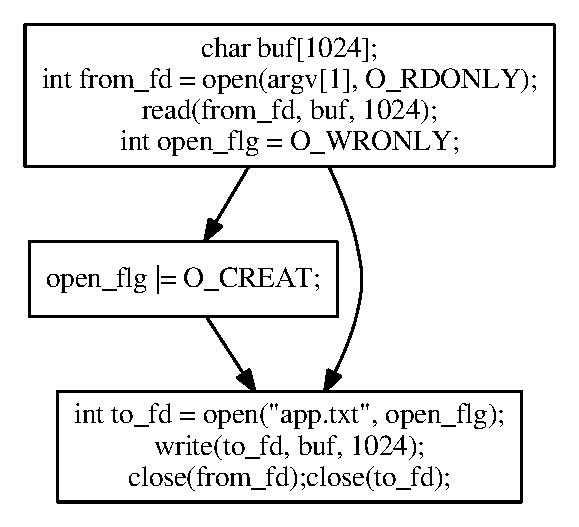
\includegraphics[width=6.0cm]{images/controlflow.eps}
    \caption{アプリケーションのコントロールフローグラフ例}
    \label{fig:controlflow}
  \end{center}
\end{figure}

この時,openシステムコールに渡される第二引数はopen\_flgは,O\_WRONLYかO\_WRONLY $|$ O\_CREAT のどちらかであることがわかる.
このような場合,O\_RDONLYやO\_RDWRを処理するコードはすべて不要であり,削除することができる.

カーネルコードのコントロールフロー解析は,アプリケーションの解析で得られたシステムコールにの引数になり得る値についての情報を利用し,switch文中の不要なcase節や不要なif文を識別するために行う.

\subsection{ブートに必要なコードの分類}
\label{propo:boot}
カーネルのソースコードには,システムコールとしてアプリケーションに提供される関数に関連するコード以外にも,多くの関数が含まれている.
デバイスを認識し初期化するコードや,マウント処理を行うコードなどである.
マシンがブートする際,カーネルはハードウェアやメモリ,ファイルシステムの初期化を行い,initプロセスを起動する.
このように,システムがブートするまでの間に,カーネルは複雑な初期化処理を行っている.
したがって,アプリケーションが必要とするシステムコールに関連するコード以外のすべてのコードを削除してしまうと,そのカーネルはブートすることができなくなってしまう.

そこで,カーネルを改変する際,ブートに必要な部分を改変しないようにする必要がある.
そのために,カーネルコードの内,ブートに必要な部分とそうでない部分を分類する.

カーネルのソースコードでは \_\_initというマクロが利用されている.
これは,kernel/include/linux/init.hとkernel/include/linux/compiler.hで,ソースコード\ref{code:__init}のように定義されている.

\begin{lstlisting}[language=C, caption=\_\_initマクロの定義, label=code:__init]
  #define __init __section(.init.text) __cold notrace
  #define __section(S) __attribute__ ((__section__(#S)))
\end{lstlisting}

これは,関数を修飾し,その関数が初期化処理用の関数であることを宣言している.
\_\_attribute\_\_修飾は,関数に特殊な属性を修飾するのに用いられるキーワードで,
この場合は,コードを配置するメモリ領域を指定するために用いられている.
\_\_initで修飾された関数は,.init.textというセクションに配置される.
.init.textセクションは初期化が終了すると廃棄されるメモリ領域である.
すなわち,\_\_initで修飾された関数はすべてブートに必要な関数であると考えられる.

また,Linuxカーネル内のinit/ディレクトリも同様に初期化に必要な処理を担当するソースコードを含んでいるため,これらもブートに必要な関数であると考えられる.

一方,これら以外にも,ファイルシステムの初期化処理など,カーネルがブート時に実行するべきコードは,Linuxカーネルソース内に広く存在している.

そこで,ブートに必要な部分の分類には,カーネルコードのカバレッジを利用する.
マシンを起動し,カーネルがブートするまでのカバレッジを取得し,そのカバレッジ情報から,ブートまでに実行されていることがわかったコードは,ブートに必要であると判断できる.
さらに,\_\_initによって修飾された関数や,initディレクトリ内の関数についても,ブートに必要なコードであると分類する.

しかし,カーネルのブートステップは非常に複雑であり,ブートまでのカバレッジ情報から分類した,ブートまでに実行されていることがわかったコードのみを残すよう,カーネルを改変しても,ブートすることが出来なかった.
そこで,本研究では,ブートに必要な関数を分類するために,一関数ずつブートするかどうかをテストする手法を提案する.

\subsection{Linuxカーネル}
\label{propo:linux}

\subsubsection{概要}
\label{propo:linux:abstruction}
カーネルは,システムの起動時にメモリにロードされ,ハードウェア資源の管理やプロセスのスケジューリングなど,オペレーティングシステムの中心的な処理を行うプログラムである.
Linuxシステムでは一般的に,/boot/ディレクトリ以下にvmlinuxやvmlinuzを名前に含むファイルに格納され,ブート時にブートローダによってメモリにロードされる.
vmlinuxは圧縮されていないカーネルである.
vmlinuzは,zlibアルゴリズムによって圧縮されたカーネルを意味し,ブートローダはこれを展開してからメモリにロードする必要がある.
また,Linuxカーネルの発展に伴うカーネルサイズの増加に対応するために,より制限の強いアーキテクチャ上であっても,展開しロードが可能なbzImageというフォーマットが作られた.
カーネルがメモリ上にロードされる際には,フォーマットに依らず,すべて展開されたvmlinuxとしてロードされる.

また,システム起動後に,必要に応じてメモリ上にロードされるモジュールという仕組みを持っており,これらは/lib/modules/ディレクトリ以下に配置される.

Linuxカーネルは,カーネルやモジュールの構成を変更するために,カーネルコンフィグレーションが可能になっている.
カーネルコンフィグレーションを行うことで,カーネルの機能の変更・追加・削除や,デバイスの変更への対応が可能となる.
コンフィグレーションによって,カーネルの機能を無効にしたり,モジュールとして外部に置きカーネル自体には組み込まないように設定できる.
Linuxカーネルのコンフィグレーションでは,使用しないデバイスのための機能を削除したり,ファイルシステムの選択を行うことができるが,
システムコールやプロセス管理などの,カーネルとしての中心的な機能を削除することは出来ない.
本研究の提案手法では,コンフィグレーションによって削除出来ない機能についても削除可能である.

Linuxカーネルのコンフィグレーションは,カーネルソースコードのルートディレクトリにある,.configというファイルを編集することで行う.
設定項目は非常に多く,アプリケーションにとって最適な構成になるよう設定するのは煩雑で難しい.

また,Linuxカーネルのビルドやブートは,非常に複雑な段階を経る.
\ref{propo:linux:compile}ではビルドについて,\ref{propo:linux:boot}ではブートについて,詳しく述べる.

\subsubsection{ビルド}
\label{propo:linux:compile}
Linuxカーネルは,ビルド時に設定ファイルを読み込むことで,様々な設定を反映したカーネルを生成する.

Linuxカーネルのコンパイルは非常に複雑なものになっている.
Linuxカーネルのソースコードには,カーネル本体のためのソースコード以外にも,カーネルイメージの圧縮や,設定ファイルや環境に合わせたコンパイルを行うためのソースコードが含まれている.
設定項目は非常に多く,それぞれの設定項目に依存関係があるものも存在する.
また,Linuxカーネルは多くのアーキテクチャをサポートしている.
そのため,環境に合わせたコンパイルを行うために,様々なツールを使用する.

例えば,Linuxカーネル内では,アーキテクチャに依存する値や設定ファイルに応じた値,コンパイルする環境に応じた値を使用する必要がある.
単純なアーキテクチャ依存の値は,arch/ディレクトリ以下の,それぞれのアーキテクチャ用のサブディレクトリ内で定義されているため,特殊な処理は不要だが,設定と関連する値などは,コンパイル時に生成しなければならない.
そこで,Linuxカーネルのコンパイルでは,まず設定ファイルを読み込み,設定依存,環境依存の値をマクロで定義するヘッダファイルをinclude/generated/ディレクトリに生成している.
実際にビルド時に生成されるファイルの一つである,include/generated/bounds.hをソースコード\ref{code:generated}に示す.

\begin{lstlisting}[language=C, caption=include/generated/bounds.h, label=code:generated]
  /*
  * DO NOT MODIFY.
  *
  * This file was generated by Kbuild
  */

  #define NR_PAGEFLAGS 25 /* __NR_PAGEFLAGS       # */
  #define MAX_NR_ZONES 4 /* __MAX_NR_ZONES        # */
  #define NR_CPUS_BITS 8 /* ilog2(CONFIG_NR_CPUS) # */
  #define SPINLOCK_SIZE 4 /* sizeof(spinlock_t)   # */

  #endif
\end{lstlisting}

include/generated/bounds.hには,環境に依存する値を定義するマクロが記述される.

また,Linuxカーネルは通常,gzipなどの圧縮アルゴリズムを用いて圧縮されている.ブート時のセットアップで,展開ルーチンが呼び出され,メモリ上に展開される.
ビルドの過程で,コンパイルされたLinuxカーネルを圧縮し,カーネルイメージを生成する.
さらに,圧縮されたカーネルを展開するルーチンも,カーネルイメージ内に含める必要がある.
Linuxカーネルを圧縮・展開するためのコードは,ソースコード内のlib/zlib\_deflate/,lib/zlib\_inflate/に含まれている.
したがって,アプリケーションが必要としていない機能のためのコードで,かつ,ブート時にも実行されないコードであっても,単純に削除することは出来ない.

それぞれのソースコード内でも特殊な記述がされている場合が多い.
通常,拡張子.cのファイルはC言語ソースコードであり,他のC言語ソースコードからインクルードされるのは,拡張子.hのヘッダファイルである.
しかし,Linuxカーネル内では,C言語ソースコードが他のC言語ソースコードをインクルードしている例がある.
kernel/bounds.cがこれに該当する.
ソースコード\ref{code:bounds}にkernel/bounds.cの内容を示す.

\begin{lstlisting}[language=C, caption=kernel/bounds.c, label=code:bounds]
/*
 * Generate definitions needed by the preprocessor.
 * This code generates raw asm output which is post-processed
 * to extract and format the required data.
 */

#define __GENERATING_BOUNDS_H
/* Include headers that define the enum constants of interest */
#include <linux/page-flags.h>
#include <linux/mmzone.h>
#include <linux/kbuild.h>
#include <linux/log2.h>
#include <linux/spinlock_types.h>

void foo(void)
{
        /* The enum constants to put into include/generated/bounds.h */
        DEFINE(NR_PAGEFLAGS, __NR_PAGEFLAGS);
        DEFINE(MAX_NR_ZONES, __MAX_NR_ZONES);
#ifdef CONFIG_SMP
        DEFINE(NR_CPUS_BITS, ilog2(CONFIG_NR_CPUS));
#endif
        DEFINE(SPINLOCK_SIZE, sizeof(spinlock_t));
        /* End of constants */
}
\end{lstlisting}

このファイル内では,関数fooの本体内で定数マクロを定義している.
本研究で提案する手法は,関数をソースコード上で削除するものであるため,関数内で定義したマクロもすべて削除されてしまう.
kernel/bounds.cが定義する定数は,このファイルをインクルードするファイルで利用されるものであるため,これらのマクロが削除されるとカーネルをコンパイルすることができない.

さらに,インラインアセンブラも多用されている.
Linuxカーネルは,非常に低レベルな処理を行う必要があるため,C言語レベルで表現できない場合がある.
例えば,プロセススケジューラ内で,実行コンテキストを切り替える処理について述べる.
切り替え前のプロセスのメモリ空間を,切り替え先のプロセスのメモリ空間に切り替え,CPUのレジスタの値を退避・復帰させる必要がある.
これを行うためには,CPUのレジスタを書き換える必要があるため,アセンブラでの記述が必要になる.
このような処理を行うために,Linuxカーネルではインラインアセンブラを利用する.
インラインアセンブラを使用しているコードに,インラインアセンブラ内で関数を定義するプログラムを記述している箇所がある.
その一つがarch/x86/kernel/kprobes/core.c内のjprobe\_return関数である.
ソースコード\ref{code:inlineasm}にその定義を示す.

\begin{lstlisting}[language=C, caption=jprobe\_return関数, label=code:inlineasm]
void jprobe_return(void)
{
        struct kprobe_ctlblk *kcb = get_kprobe_ctlblk();

        asm volatile (
#ifdef CONFIG_X86_64
                        "       xchg   %%rbx,%%rsp      \n"
#else
                        "       xchgl   %%ebx,%%esp     \n"
#endif
                        "       int3                    \n"
                        "       .globl jprobe_return_end\n"
                        "       jprobe_return_end:      \n"
                        "       nop                     \n"::"b"
                        (kcb->jprobe_saved_sp):"memory");
}
\end{lstlisting}

インラインアセンブラ内で,jprobe\_return\_endという関数を定義している.
このようなインラインアセンブラ内での関数定義を含む関数を削除してしまうと,リンク時にエラーになってしまう.
関数の宣言が存在するにもかかわらず,バイナリにその関数の実態が生成されないためである.
また,インラインアセンブラ内で定義された関数は,そのカバレッジ情報が生成されない.
このような関数のカバレッジ情報は,インラインアセンブラを含む関数のカバレッジ情報として計測される.

Linuxカーネルは,汎用目的のカーネルであるため,非常に複雑なソフトウェアであり,様々なアーキテクチャ,設定に対応する必要がある.
そのために,ビルド手順も非常に複雑になっていることがわかる.

\subsubsection{ブート}
\label{propo:linux:boot}

\ref{propo:linux:abstruction}で述べたように,Linuxカーネルは圧縮された形式でファイルに置かれる.
x86アーキテクチャでは,デフォルトではbzImage形式にされたカーネルイメージが生成される.
bzImageは,setup.binとvmlinux.binというバイナリを連結したものである.
setup.binはカーネルイメージの先頭に存在し,エントリーポイント\_startを含む.
このエントリーポイントから開始されるコードによって,圧縮されたカーネルを展開するルーチンが起動される.
vmlinux.binは,圧縮されたカーネル本体と,その展開ルーチンを含むバイナリである.

マシンが起動すると,まずBIOSというソフトウェアが起動する.
BIOSは,ハードウェアを初期化し,ブートデバイスを決定し,ブートローダを実行する.
ブートローダとは,記憶媒体に書き込まれているカーネルを,メモリ上に展開するためのソフトウェアである.
Linuxでは,カーネルも通常のファイルのように,ファイルシステム上に格納されており,また,様々なファイルシステムに対応しているため,BIOSが直接カーネルファイルをロードすることは出来ない.
代表的なブートローダには,LILO,SYSLINUX,GRUB,GRUB2などが挙げられる.

ブートローダは,vmlinuzやbzImageの形式になっているカーネルイメージを解釈し,展開する.
bzImageの場合,bzImage内に含まれる展開ルーチンを呼び出し,圧縮されたカーネルを展開する.
カーネルが展開され,メモリ上にロードされると,ブートローダはカーネルへと処理をうつす.

展開されたカーネルへと処理がうつった後,ハードウェアの極低レベルな初期化処理や,メモリ管理の開始が行われる.
このステップまでステップでは,その処理のほとんどがアセンブラで記述されており,本研究での改変の影響を受けにくい.
本研究では,C言語レベルでの関数単位での改変のみを行っているためである.

ハードウェアの極低レベルな初期化処理やメモリ管理が開始された後,setup\_kernel関数が呼び出される.
この関数はC言語で記述されており,initプロセスを起動するまでのカーネル環境の初期化を行う.
setup\_kernel関数はまず,環境依存の初期化処理を行う関数を呼び出す.
その後,メモリアロケータの初期化,スケジューラの初期化・起動,割り込みの処理,デバイスドライバの初期化,ファイルシステムの初期化,initプロセスの起動準備を行う.

Linuxカーネルのブートは,環境やタイミングによって実行される関数が異なる.
ハードウェアの認識,初期化処理は,ブートするマシンの利用しているハードウェアに応じて異なる処理になる.

本研究では,カーネルコードカバレッジを用いてブートに必要な部分の識別を行うことを提案しているが,
ブートの極初期の段階では,カバレッジ情報を書き込むファイルシステムのセットアップが終わっておらず,
その段階でしか実行されないコードは正しく分類できないと考えられる.
そのため,ブートに必要となる部分だけを正確に分類することは非常に難しい.


\clearpage
\section{実装}
\label{implementation}
\subsection{概要}
\label{implementation:abstruction}
提案手法を実装するためには,第\ref{proposal}章で述べた通り,まず,Linuxカーネルのソースコードの内,ブートに必要となる部分を識別する必要がある.
本研究では,Linuxカーネルのブートに必要となる部分を識別する方法を,三種類の手法で実装した.

すべての手法に共通して,Linuxカーネルのコードカバレッジを用いて,ブートに不要であると思われる関数名を取得する.
次に,Linuxカーネルのソースコードを構文解析し,ブートに不要であると思われる関数を削除する.

手法1では,コードカバレッジから,ブート時に実行されていたことがわかった関数以外のすべての関数を削除した.
手法2では,コードカバレッジから,ブート時に一度も実行されていなかった関数をすべて削除した.
手法3では,コードカバレッジから,ブート時に一度も実行されていなかった関数を,一つずつ削除し,ブート可能なカーネルを生成できるかテストする環境を構築した.


\subsection{ブートに必要な部分の識別}
\label{implementation:boot}
ブートに必要な部分を識別するためには,Linuxカーネルのコードカバレッジを利用する.
コードカバレッジとは,プログラムのソースコード全体に対する実行されたコードの割合を示し,通常はソフトウェアのテストがプログラム全体の内,どれだけのコードをテストできているかを示す指標として使われる.
Linuxブート直後のコードカバレッジを解析し,一度も実行されていないコードは,ブートに不要な関数であると判定できる.

コードカバレッジの取得には,gcovを用いる.
gcovとは,GNU CCと合わせて使用する,プログラムのコードカバレッジを取得するツールである.
\texttt{gcc -coverage main.c}のようにコンパイルすると,\texttt{main.gcno}というファイルと実行ファイルが生成される.
生成された実行ファイルを実行すると,\texttt{main.gcda}というファイルが生成され,\texttt{gcov main.c}とコマンドを実行するとプロファイル結果が出力される.
プロファイル結果の例をソースコード\ref{code:gcov}に示す.

\begin{lstlisting}[caption=gcovの実行結果例, label=code:gcov]
        -:    0:Source:main.c
        -:    0:Graph:main.gcno
        -:    0:Data:main.gcda
        -:    0:Runs:1
        -:    0:Programs:1
        1:    1:int f(void)
        -:    2:{
        1:    3:  return 0;
        -:    4:}
        -:    5:
        1:    6:int g(int x)
        -:    7:{
        1:    8:  if (x > 0)
    #####:    9:    return x;
        -:   10:  else
        1:   11:    return -x;
        -:   12:}
        -:   13:
    #####:   14:int h(void)
        -:   15:{
    #####:   16:  return 0;
        -:   17:}
        -:   18:
        1:   19:int main(void)
        -:   20:{
        1:   21:  int x = f();
        1:   22:  int y = g(x);
        1:   23:  return 0;
        -:   24:}
\end{lstlisting}

$:$の右側に,対象となるソースコードが,
$:$の左側に,その行が何度実行されたかが示されている.
ソースコード\ref{code:gcov}の例であれば,関数gのif文の分岐の片方が実行されていないことがわかる.
また,関数hが一度も実行されていないことがわかる.

gcovは,Linuxカーネルと組み合わせることが可能で,Linuxカーネルのビルド設定を変更し,gcovを組み込むことで,カーネルコードのカバレッジが取得できる.
本研究では,Linuxマシンをブートさせた直後のコードカバレッジを利用することで,Linuxカーネルコードのどの部分がブートに必要であるかを判定する.
ブート直後のコードカバレッジで,一度も実行されていないコードはブートプロセスにとって不要であると言える.

Linuxカーネルにgcovを組み込むためには,カーネルのビルド設定をソースコード\ref{code:gcovkernel}のように設定する.

\begin{lstlisting}[caption=gcovを組み込むLinuxカーネルの設定, label=code:gcovkernel]
  CONFIG_DEBUG_FS=y
  CONFIG_GCOV_KERNEL=y
  CONFIG_GCOV_PROFILE_ALL=y
\end{lstlisting}

Linuxカーネルのカバレッジを取得するためには,debugfsをマウントする必要がある.
debugfsとは,Linuxカーネルの内部情報をユーザが参照するための,メモリ上に存在するファイルシステムで,\texttt{mount -t debugfs /sys/kernel/debug}コマンドを実行することでマウントできる.
このようにdebugfsをマウントすると,/sys/kernel/debug/gcov/以下にLinuxカーネルのカバレッジ情報を保持するファイルとソースコードとの対応をとるためのファイルへのシンボリックリンクが生成される.
ソースコードとの対応を取るためのデータファイルであるgcnoファイルの実体は,Linuxカーネルをビルドしたディレクトリ以下に配置されている.
また,/sys/kernel/debug/gcov/resetというファイルも生成されており,このファイルに書き込みを行うと,カバレッジ情報をリセットすることができる.
そこで,/sys/kernel/debug/gcov/resetへ書き込みを行った直後にシステムをリブートし,ブートが終了したタイミングでカバレッジ情報を収集する.

本研究では,gcovのカバレッジ情報から,関数単位での実行回数を取得する.
\texttt{gcov}コマンドのオプションで,\texttt{-f}を指定すると,関数単位でのプロファイル結果が出力される.
ソースコード\ref{code:gcov}で示したプログラムについて,\texttt{gcov -f main.c}を実行した際の出力を,ソースコード\ref{code:gcovfunction}に示す.

\begin{lstlisting}[caption=関数単位でのプロファイル結果, label=code:gcovfunction]
% gcov -f main.c
Function 'f'
Lines executed:100.00% of 1

Function 'g'
Lines executed:75.00% of 4

Function 'h'
Lines executed:0.00% of 1

Function 'main'
Lines executed:100.00% of 3

File 'main.c'
Lines executed:77.78% of 9
main.c:creating 'main.c.gcov'
\end{lstlisting}

ソースコード\ref{code:gcovfunction}が示すように,関数名と,その関数本体の行数に対する実行された行数の割合が表示される.
ソースコード\ref{code:gcovfunction}から,関数hが一度も実行されていないという結果が得られる.

Linuxカーネルのブート時に一度も実行されない関数を取得するために,ブート直後のカバレッジ情報を用いる.
その際,ブート時には実行されないが,デーモンを起動するために実行されたり,デーモンが実行するコードを,ブートに必要なコードであると判定することがないよう,ブート直後に起動するデーモンはすべて無効にしておく必要がある.
Linuxカーネル内の,すべてのソースコードに対して,\texttt{gcov -f}コマンドを実行し,出力結果をパースして,実行された割合が0.00%だった関数名をすべて取得する.

また,gcovを組み込んだカーネルは,カバレッジ情報を蓄積しながら実行されるため,非常に動作が重くなる.
そこで,ブートに必要なコードの調査時にはgcovを組み込んだカーネルを使用するが,それを基に改変したLinuxカーネルのビルド時にはgcovを無効にすることを目標にする必要がある.
改変後のカーネルには,アプリケーションを実行する機能のみをもたせるべきであり,カバレッジの取得は不要なためである.

\subsection{関数の削除}
\label{implementation:function}
gcovを用いて得た,ブートに不要と思われる関数を,Linuxカーネルから削除するために,Linuxカーネルのソースコードを構文解析し,得られた関数の定義されている行と列を調べる必要がある.
Linuxカーネルの構文解析には,clang\cite{clang}の提供するLibToolingを用いる.

clangとは,C言語,C++,Objective-C,Objective-C++用のコンパイラフロントエンドである.バックエンドにはLLVMを採用している.
clangは,これらのプログラミング言語で書かれたソースコードを,構文解析し,抽象構文木に変換する.
変換された抽象構文木には,コンパイルの構文解析以降でプログラムの誤りを検知した際のエラー通知のために,ソースコード中の位置情報が含まれている.
また,型検査やコントロールフロー解析など,様々な静的解析を実装している.

clangの提供するLibToolingというライブラリは,clangをベースにしたツールを支援するためのライブラリである.
これを利用することで,clangに構文解析を任せることができ,抽象構文木に変換されたソースコードにアクセスすることができる.
本研究では,C言語で記述されたソースコードをclangに構文解析させ,そのソースコード内で定義されている関数の名前と,それぞれの関数の定義されているソースコード上の位置情報を取得するために,LibToolingを利用する.

gcovによるプロファイル結果をパースし,ブートに不要と思われる関数を,その関数の定義されているファイル名と合わせて出力する.
ファイル名と関数名から,LibToolingを用いて実装したツールを用いて,ファイル名,関数本体の開始位置,関数本体の末尾位置を取得する.
ソースコード\ref{code:gcov}の例の関数hの場合,7行目1列目が開始位置で,12行目1列目が末尾位置という結果が得られる.

得られた開始位置と末尾位置の間のコードを,ソースコード\ref{code:before},ソースコード\ref{code:after}に示したように書き換える.
関数の定義そのものをすべて削除してしまうと,カーネルのコンパイルがエラーになってしまう.
そこで,関数の定義自体は残し,関数の先頭ですぐにpanic関数を呼び出すように変更する手法を取る.

panic関数は,Linuxカーネルをパニックさせる関数である.Linuxカーネルがパニックすると,Linuxカーネルは,パニックしたというメッセージと,パニックした原因,パニック時のダンプ情報の一部を出力する.
panic関数の引数には,パニックした原因として出力されるメッセージを指定する.
ソースコード\ref{code:after}に示すように,panic関数の引数には,改変対象となっている関数の定義されているファイル名と,その関数の名前を含む文字列を指定する.
ソースコード\ref{code:after}のようにpanic関数を呼び出すことで,改変したカーネルが削除した関数を呼び出してしまった場合に,その場で適切なエラーメッセージを表示するようパニックさせることができる.

また,panic関数の呼び出しを\texttt{\#ifdef \_LINUX\_KERNEL\_H}と\texttt{\#endif}で囲んでいるのは,Linuxカーネルのビルド時にコンパイルエラーが生じることを防ぐためである.
panic関数は,include/linux/kernel.hで宣言されている.
Linuxカーネルソースコード中の,すべての関数がこのファイルをインクルードしているとは限らないため,panic関数が前方宣言されていることを確認する必要がある.

clangにC言語ソースコードを構文解析させる際,カバレッジ情報から取得した関数名を持つ関数の定義を発見できない場合がある.
コードカバレッジから解析した,ブート時に一度も実行されていない関数名の一部を表\ref{table:unusedfunctions}に示す.

\begin{table}[H]
\begin{center}
  \begin{tabular}{ll} \hline
    ファイル名 & 関数名 \\ \hline \hline
    ipc/shm.c & shm\_add\_rss\_swap.isra.15 \\
    ipc/shm.c & sysvipc\_shm\_proc\_show \\
    kernel/sysctl.c & warn\_sysctl\_write.isra.1 \\
    kernel/sysctl.c & proc\_do\_large\_bitmap \\
    kernel/sysctl.c & proc\_do\_cad\_pid \\ \hline
  \end{tabular}
  \caption{ブート時に実行されていなかった関数(一部)}
  \label{table:unusedfunctions}
\end{center}
\end{table}

表\ref{table:unusedfunctions}に示されているように,gcovの出力するカバレッジ情報には,C言語の関数名として有効でない関数名を持つ関数が数多く出力されている.
"関数名\_isra.XXX"という形式になっているものは,Linuxカーネルのビルドに用いたC言語コンパイラのgcc\cite{gcc}が,関数を最適化する際に,".\_isra.XXX"という接尾語を関数名に付与したものである.
この最適化は,gccのコンパイルオプション\texttt{-fipa-sra}が指定されるか,最適化のためのオプションである,\texttt{-O2},\texttt{-O3},\texttt{-Os}が指定された場合に,実行される最適化である.
ポインタを通じた参照渡しによる関数呼び出しを,参照渡しにする必要がない場合に,値渡しによる関数呼び出しに変更する最適化である.

Linuxカーネルは,通常\texttt{-O2}というオプションでコンパイルされるため,この最適化が有効になっている.
カーネルコンフィグレーションによって,\texttt{CONFIG\_CC\_OPTIMIZE\_FOR\_SIZE}が指定されている場合でも,\texttt{-Os}が有効になる.
この最適化は,
最適化によって関数が書き換えられる際に,関数名が変更される.
このような場合,C言語のソースファイルを構文解析しても,関数を見つけることが出来ない.
C言語のソースファイル上で定義されている関数名は,".\_isra.XXX"という接尾語が付与される前のものである.

さらに,Linuxカーネルのコンパイルは,gccの最適化に依存したコードを含んでおり,最適化を無効にすることが出来ない.
したがって,バイナリになったLinuxカーネルは,最適化の影響を大きく受けており,関数名の改変など,カバレッジ情報へも影響が及んでいる.

構文解析によってその関数の定義を発見できなかった場合,その関数の削除は行えない.
しかし,最適化によって関数の定義が発見できなくなる場合については,大きな問題にはならない.
なぜなら,gccの最適化によって生成された関数は,元となった関数自体が削除されたり,その最適化を行う原因となった関数呼び出しを行っている関数が削除された場合,生成されなくなるためである.

\subsection{手法1}
\label{implementation:1}

手法1は,コードカバレッジから,ブートに必要であるとわかった関数以外のすべての関数を削除する手法である.
\ref{implementation:boot},\ref{implementation:function}で述べた方法で,コードカバレッジからブートに必要であるとわかった関数以外のすべての関数を削除した.
ソースコード\ref{code:impl1}に擬似コードを示す.

\begin{lstlisting}[language=ruby, caption=手法1の擬似コード, label=code:impl1]
  # ブートに必要な関数名の集合
  necessary_functions = {}

  # ブートに必要な関数名一覧をコードカバレッジから取得する
  for file in Linuxカーネルのカバレッジ情報をもつすべてのファイル
    for function in fileがカバレッジ情報を持つすべての関数
      if function の実行率が0%でない
        neccesary_functions << function
      end
    end
  end

  # ブートに必要な関数以外をすべて削除する
  for file in Linuxカーネルソース内の拡張子が.cであるすべてのファイル
    for function in file内で定義されているすべての関数 
      if function が neccesary_function に含まれない
        function をpanic関数呼び出しへ置き換える
      end
    end
  end
\end{lstlisting}

この手法で改変したLinuxカーネルのビルドを試みたところ,ビルドすることが出来なかった.
\ref{propo:linux:compile}で述べたように,Linuxカーネルのビルドは複雑なステップを経る.
この手法では,ビルド時に環境に依存した値を定義するヘッダファイルを生成するためのツールのソースコードやそのためのライブラリコード,複数のファイルの間で必要になるマクロの定義などをすべて削除してしまう.
これらは,ビルド時にのみ使用され,Linuxカーネル本体には組み込まれないためである.
gcovが出力するカバレッジ情報は,実際にLinuxカーネルのバイナリに含まれている関数の情報のみであるため,ビルド時にのみ必要となるコードに関しては,カバレッジが出力されず,削除すべきと判断されてしまう.
実際に,これらのコードの多くは,Linuxカーネルのブート時には実行されない.
しかし,Linuxカーネル本体に組み込まれないコードを削除しても,カーネルのサイズを削減することはできず,意味がない.

また,gcovでは,Linuxカーネルのバイナリに含まれるコードの実行回数などのプロファイルを測定できるが,Linuxカーネルソースコード中のマクロが使用されたかどうかは測定することは出来ない.
C言語におけるマクロは,すべてコンパイルの前の段階でプリプロセッサによって解決され,コンパイル後のバイナリには現れないためである.
したがって,ある関数内で定義したマクロが,他の関数や他のソースコード中で使用されていたとしても,それをgcovを用いて検知することは出来ない.
他の関数でも使用されるマクロを,関数本体の定義内で定義していても,その関数がバイナリとして実行されていない場合,マクロごと関数の定義を改変してしまう.

手法1の結果から,Linuxカーネルのビルドが非常に複雑なステップを踏んでおり,ビルド時にのみ使用するツールやライブラリのコードを多く含むことがわかった.

\subsection{手法2}
\label{implementation:2}
手法2は,コードカバレッジから,ブートに不要であるとわかった関数のみをすべて削除する手法である.

手法2では,gcovによって得られるコードカバレッジが,Linuxカーネル本体に組み込まれている関数のプロファイル結果しか出力していないことに着目した.
手法2の擬似コードをソースコード\ref{code:impl2}に示す.

\begin{lstlisting}[language=ruby, caption=手法2の擬似コード, label=code:impl2]
  for file in Linuxカーネルソース内の拡張子が.cであるすべてのファイル
    if file のカバレッジ情報が出力されている
      for function in file内で定義されているすべての関数
        if functionの実行率が0%である
          functionの定義をpanic関数呼び出しへ置き換える
        end
      end
    end
  end
\end{lstlisting}

コードカバレッジの解析結果から,ブート時に一度も実行されていないとわかった関数は,必ずLinuxカーネル本体に組み込まれている.
一方で,ビルド時にのみ利用されるようなツールのためのソースコードはLinuxカーネル本体には組み込まれないため,プロファイル結果が出力されない.
そこで,ソースコード\ref{code:impl2}に示すように,カバレッジ情報が出力されたファイルについてのみ書き換えを行い,カバレッジ情報が出力されなかったファイルについては改変を行わない.

手法1で,カーネルのビルドに失敗してしまう原因をビルド時のエラーメッセージから調査したところ,エラーの要因となりうる箇所が非常に多く,事前に発見するのが困難であることがわかった.
そこで,手法2のように,Linuxカーネル本体に組み込まれている関数のみを対象に改変を行う方法を取った.

この手法で改変したLinuxカーネルは,ビルドすることができなかったが,手法1と異なり,ビルドステップの多くの部分は問題なく成功していたため,ビルドが失敗する原因をすべて調査することができた.
ソースコード\ref{code:inlineasm}に示したような,関数定義内のインラインアセンブラで関数を定義している関数や,lib/zlib\_inflateディレクトリ以下のソースコードのような,カーネルの圧縮展開のためにビルド時にもカーネル本体にも使用される関数が原因であることがわかったため,これらを書き換えないよう変更したところ,カーネルのビルドに成功した.

また,\ref{implementation:boot}で述べたように,gcovを組み込んだLinuxカーネルは非常に動作が重くなるため,改変したカーネルをgcovを無効にするカーネルコンフィグレーションでもビルドした.
gcovを組み込んだ場合と同様の例外が生じたが,gcovを無効にする場合であっても,カーネルのビルドは成功した.

しかし,このカーネルを用いたブートは,gcovの設定にかかわらず,不可能だった.
ブートに失敗しても,どの部分の改変が問題となっているかがわかるよう,関数を削除する際には,ソースコード\ref{code:after}が示すようにpanic関数を呼び出すように改変を加えていたが,実際にはパニックメッセージを確認することが出来なかった.
また,ブートに失敗する原因を調査するため,Linuxカーネルのパラメータ設定を用い,パニックが発生した場合自動的にリブートするよう設定したが,リブートすることもなかった.
これは,ブートの非常に初期の段階で問題が発生しているために,パニックメッセージの出力やリブートが正常に行えなかったと考えられる.

手法2で生成したカーネルがブートに失敗するのは,ブート時に実際には必要であるが,不要と誤判定され,改変されてしまった関数が原因である.
そこで,gcovによるカバレッジとは別に,Linuxカーネルがブート時に呼び出すと思われる関数を調査した.
\ref{propo:boot}に示した,\texttt{\_\_init}が指定されているコードや,init/ディレクトリ以下にあるソースコードは,ブート時の初期化処理のために使用される可能性が高いため,改変しないように変更した.
しかし,initを除外したルールで改変したカーネルも,ブートさせることができなかった.

原因となる関数を探すため,Linuxカーネルソースツリーの各ディレクトリについて,そのディレクトリのみを改変するという実験を行った.
図\ref{fig:directory}に示す.

\begin{figure}[H]
  \begin{center}
    \includegraphics[width=10.0cm]{images/boottest.png}
    \caption{Linuxソースツリーの各ディレクトリごとの改変を行った場合のブート可否}
    \label{fig:directory}
  \end{center}
\end{figure}

図\ref{fig:directory}から,ほとんどのディレクトリは,改変を単純に行うとブートが失敗してしまうことがわかる.
したがって,ブートに失敗する原因となる関数は広く点在しており,それらを特定して手法2に例外規則を追加しブート可能なカーネルを生成するのは難しい.

また,lib/ディレクトリ以下の各ファイルについて,改変を行った場合のブートの可否を調査したところ,220ファイルのC言語ソースコードの内,72ファイルは改変するとブートができなくなることがわかった.
実際にはファイル中の関数単位での改変を行っているため,この結果より安全に改変を行える可能性は高い.さらにlib/ディレクトリは,様々なコードから利用されるライブラリのためのコードを多く含むため,実行される可能性が高い関数が,他のディレクトリと比較して,より多いことが考えられる.
しかし,これをすべてのディレクトリについて行うのは現実的とは言えない.
Linuxカーネルは大量のソースコードを含むためである.


\subsection{手法3}
\label{implementation:3}
手法3は,ブート時に不要と思われる関数それぞれについて,panic関数への置き換えとブート可能かどうかのテストを行う手法である.
擬似コードを,ソースコード\ref{code:impl3}にしめす.

\begin{lstlisting}[language=ruby, caption=手法3の擬似コード, label=code:impl3]
  # ブート時に不要と思われる関数名の集合
  unneccesary_functions = {}

  # ブートに不要な関数名一覧をコードカバレッジから取得する
  for file in Linuxカーネルのカバレッジ情報をもつすべてのファイル
    for function in fileがカバレッジ情報を持つすべての関数
      if function の実行率が0%である
        unneccesary_functions << function
      end
    end
  end

  # ブート時に不要と思われる関数それぞれについて,
  # 改変とブートのテストを行う.
  for function in unneccesary_functions
    file = functionが定義されているファイル
    # ファイルのバックアップを取る
    backupfile = file + "backup"
    copy(from: file, to: backupfile)

    functionの定義をpanic関数呼び出しへ置き換える
    カーネルをビルドする

    if カーネルのビルドが失敗
      # バックアップから復元
      move(from: backupfile, to: file)
      # 次の関数へ
      continue
    end

    カーネルをブートする

    if カーネルのブートが失敗
      # バックアップから復元
      move(from: backupfile, to: file)
      # 次の関数へ
      continue
    end
  end
\end{lstlisting}

手法2の分析結果から,ブートに必要な関数をすべて正確に取得することが非常に困難であることがわかる.
コードカバレッジでは,実行率0%という結果になっている関数であっても,コンパイラの最適化の影響によって,実際には必要であるにもかかわらず,実行率0%になる場合がある.
ブートの手順は非常に複雑なため,手動での分類は困難であり,また,コードカバレッジから単純に不要な関数を分類することも出来ない.
そこで,手法3では,手法1,手法2の結果を踏まえて,カーネルがブートすることをテストしながら,関数を削除していく方法を取った.

カーネルのブートの成否は,一台のマシンではテストすることができない.
ブートに失敗した場合,通常はパニックが発生するが,パニックが発生した後,その結果を通知する方法がない.
また,本研究でテストの対象としたいカーネルは,関数をあs駆除するという改変を行っているため,パニックを正常に発生させることができるという保証がない.
そこで,本研究では,仮想マシンを二台用いて,一方でもう一方を監視するという手法をとる.

マシンを二台用いたカーネルのテストには,ktest.plというperlで記述されたスクリプトを用いる.
ktest.plは,Linuxカーネルソースツリーに含まれるスクリプトで,設定ファイルを基にカーネルのテストを行う.
ビルドやブートが正常に行えるかをテストすることができる.
通常,ktest.plは,Linuxカーネルの開発時にカーネルのテストを自動化するためのツールで,テスト対象のカーネルがパニックしたりハングアップした場合であってもテストを継続することができる.
テストには,ホストマシンとターゲットマシンの二台が必要である.
ホストマシンは,テスト対象のカーネルをビルドし,ターゲットマシン上のテストの進行を監視する.
ターゲットマシンは,テスト対象のカーネルを実行するマシンで,ホストマシンから電源の切り替えが可能で,ホストからコンソールに接続ができ,rootユーザとしてsshでホストから接続できる必要がある.

仮想マシンの構成では,OpenStackというクラウド基盤ソフトウェアを用いる.
OpenStackは,オープンソースソフトウェアのクラウド基盤ソフトウェアで,高信頼なプライベートクラウド基盤を構成することができる.
OpenStackを用いて構成したクラウド基盤上に,ブートテスト用の仮想マシンとビルド用の仮想マシンを用意する.カバレッジの解析とカーネルのビルドをビルド用マシンで行い,生成されたカーネルをブートテスト用マシンに転送する.
OpenStackを用いて構成した実装環境を図\ref{fig:openstackenv}に示す.

\begin{figure}[H]
  \begin{center}
    \includegraphics[width=10.0cm]{images/openstackenv.png}
    \caption{OpenStackを用いて構成した実装環境}
    \label{fig:openstackenv}
  \end{center}
\end{figure}

改変の対象となるLinuxカーネルには,Linux-4.2.3を用いた.
また,OpenStack上の仮想マシンには,Ubuntu 12.04を用いた.

ktest.plは,カーネルのビルド,転送,ブート,結果の取得を自動化する.
カーネルの転送には,scpを用いる.
ブートテスト用マシン上でコマンドを実行するために,rootユーザとしてsshを利用する.
転送されたカーネルを,/boot/ディレクトリ以下に配置し,そのカーネルを使用するよう設定してからリブートする.
この際,常に改変されたカーネルを使用してブートするようにブートテスト用マシンを設定してしまうと,そのカーネルがブートできないカーネルだった場合,sshでコマンドを実行したり,scpでファイルを転送することができなくなってしまう.
これを解決するために,ブートローダであるgrubが持つ,grub-rebootというコマンドを用いる.
grub-rebootは,次の一度のリブートのみを有効期限とする設定を行うコマンドである.
grub-rebootを用いて,一度だけ改変カーネルを使用してブートするように設定することで,そのカーネルがブート不可能なものだった場合でも,もう一度リブートすることで,通常のカーネルを使用したブートが可能になる.

通常,ktest.plを利用する場合は,そのスクリプト本体を書き換えることなく,設定ファイルによって,テストの内容を変更できる.
本研究では,OpenStack上でktest.plを使用するために,ktest.plをOpenStackに合わせるよう書き換える必要がある.
ktest.plは,ブートテスト用のマシンのコンソール出力を読み込み,ログインプロンプトが出力されていればブートに成功したと判定する.
OpenStack上の仮想マシンのコンソール出力は,リモートシリアルコンソールが利用できないため,ktest.plは,テスト用マシンの出力を読み込むことが出来ず,ブートに成功したかどうかを判定することが出来ない.
そこで,OpenStackクラウド上のリソースの管理のためのCompute APIをコマンドラインから操作する,novaクライアントを用いる.
novaクライアントを用いることで,ブートテスト用マシンのコンソールの出力を,ktest.plが読み取ることが可能になる.
また,改変したカーネルのブートの成否にかかわらず,ブート確認の後,ブートテスト用マシンを通常のカーネルを用いてリブートする必要がある.
このリブートには,rebootコマンドは使用できない.ブートに失敗している可能性があるためである.
ブート確認後のリブートにも,novaクライアントを用いる.

ktest.plを利用するためには,ブートテスト用マシンに,ktest用のgrubエントリーを作成する必要がある.
ktest用のgrubエントリーでは,ビルド用マシンから転送されてきたカーネルを使用してブートするよう設定する.
ビルド用マシン側では,カーネルをビルドした後,ブートテスト用マシンにscpを用いてカーネル本体とカーネルモジュール群を転送し,sshでこれらをブートできるよう移動する.
この際,sshで/boot/ディレクトリ以下への書き込みを行う必要があるため,ビルド用マシンからブートテスト用マシンへは,rootユーザとしてsshでアクセス可能にしなければならない.

図\ref{fig:openstackenv}のように,OpenStack,ktest.pl,novaクライアントを用いて構成した環境で,実際にLinuxカーネルの改変を進めたところ,正しくブートの可否の判定が行えることがわかった.

\clearpage
\section{分析結果}
\label{result}

Linuxカーネルのブートまでのコードカバレッジをgcovを用いて解析したところ,カーネルソースコードの大部分が,ブートまでには実行されないことがわかった.
\ref{implementation:3}で示した,OpenStackを用いたテスト環境上で,ブート直後のカバレッジから,一度も実行されていない関数を解析したところ,コードカバレッジが出力されていた関数が56462個あり,その内41370個の関数が一度も実行されていないことがわかった.
したがって,ブートができる最小のカーネルには,通常のLinuxカーネルの約73%の関数が不要であるといえる.

しかし,実際にはそれらの関数をすべて削除すると,カーネルがブートしなくなってしまうことがわかった.
これは,コンパイラの最適化による影響と考えられる.
Linuxカーネルのコンパイルに用いるgccでは,様々な最適化を施したコードを生成することができる.
通常,Linuxカーネルは最適化を有効にした状態でコンパイルされる.

gccの施す最適化の一つに,インライン展開がある.
インライン展開とは,関数呼び出しを,その関数の本体をインラインに展開することで置き換える最適化である.
例えば,ソースコード\ref{code:inlinefunction}をコンパイルする場合を考える.

\begin{lstlisting}[language=C, caption=インライン展開のコード例, label=code:inlinefunction]
  int f(int x)
  {
    return ++x;
  }

  int main(int argc, char** argv)
  {
    int c = f(argc);
    printf("%d\n", c);
    return 0;
  }
\end{lstlisting}

ソースコード\ref{code:inlinefunction}を最適化を無効にしてコンパイルした結果の一部をソースコード\ref{code:nooptimized}に,最適化を有効にしてコンパイルした結果の一部をソースコード\ref{code:optimized}に示す.

\begin{lstlisting}[language={[x86masm]Assembler}, caption=最適化を無効にしたコンパイル結果, label=code:nooptimized]
main:
	pushq	%rbp
	movq	%rsp, %rbp
	subq	$32, %rsp
	movl	%edi, -20(%rbp)
	movq	%rsi, -32(%rbp)
	movl	-20(%rbp), %eax
	movl	%eax, %edi
	call	f
	movl	%eax, -4(%rbp)
	movl	-4(%rbp), %eax
	movl	%eax, %esi
	movl	$.LC0, %edi
	movl	$0, %eax
	call	printf
	movl	$0, %eax
	leave
	ret
\end{lstlisting}

\begin{lstlisting}[language={[x86masm]Assembler}, caption=最適化を有効にしたコンパイル結果, label=code:optimized]
main:
	leal	1(%rdi), %esi
	subq	$8, %rsp
	movl	$.LC1, %edi
	xorl	%eax, %eax
	call	printf
	xorl	%eax, %eax
	addq	$8, %rsp
	ret
\end{lstlisting}

ソースコード\ref{code:inlinefunction}では,関数fの内部で整数の演算を行い,その結果を関数printfを用いて出力している.
インライン展開の様子がわかりやすくなるよう,定数の畳込みなどの他の最適化が適用されないよう,実行時まで決定されないargcを用いた演算を行っている.

最適化を無効にした場合,\texttt{call f}という行が結果にあらわれている.
\texttt{call}は,関数呼び出しを行う命令であり,\texttt{call f}は,関数fの呼び出しを行う命令である.
関数fを呼び出した後,関数printfを呼び出していることがわかる.
一方,最適化を有効にした場合は,関数fの呼び出しが行われず,関数printfが呼び出されていることがわかる.
これは,関数fの内部で行う演算を,main関数の内部にインライン展開するという最適化が施された結果である.

gcovによるコードカバレッジには,このような最適化の影響が反映されてしまう.
ソースコード\ref{code:inlinefunction}を,最適化を有効にしてコンパイルし,実行した場合のコードカバレッジを,ソースコード\ref{code:inlinecoverage}に示す.

\begin{lstlisting}[caption=最適化を有効にした場合のgcovの出力, label=code:inlinecoverage]
Function 'main'
Lines executed:100.00% of 3

Function 'f'
Lines executed:0.00% of 1

File 'calc.c'
Lines executed:75.00% of 4
\end{lstlisting}

ソースコード\ref{code:inlinefunction}では,明らかに関数fを一度呼び出しており,最適化を有効にした場合であっても,実行結果は正常である.
しかし,gcovの出力するカバレッジ情報では,関数fの実行率が0%になってしまっている.
これは,インライン展開によって,関数fの呼び出し自体が最適化され,削除されているためである.

関数がインライン展開され,その関数を呼び出すコードが削除された場合でも,実際にはその関数の定義は必要である.
ソースコード\ref{code:inlinefunction}の例では,関数fの定義を改変すると,インライン展開後のコードも改変されてしまう.

gccでは,インライン展開以外にも,\ref{implementation:function}で示した,ipa-sra最適化など,様々な最適化が施され,
それらgcovの出力するカバレッジ情報に影響を及ぼすことがわかった.
したがって,Linuxカーネルのブートに必要なコードを,コードカバレッジから取得する場合には,これらの最適化をすべて無効にしなければならないことがわかった.

Linuxカーネルビルド時の最適化オプションは,Linuxカーネルソースツリー内のMakefileで,\texttt{KBUILD\_CFLGAS}という変数に定義されており,
通常は\texttt{-O2}が指定されている.
この値を\texttt{-O0}に変更することで,最適化を無効にすることができる.
しかしながら,Linuxカーネルは,GCCの最適化に依存したコードを含んでおり,Linuxカーネルを,最適化を無効にした状態でコンパイルすることは出来ない.
したがって,\ref{implementation:3}で示すような,自動的にブートの可否をテストできる環境が必要であることがわかった.

\ref{implementation:3}で示した,OpenStack上に構築した二台の仮想マシンによる,ブートの自動テストと自動改変は,非常に時間がかかる.
これは,一つの関数を書き換えるたびに,カーネルのビルド,カーネルの転送,ブートの確認を行う必要があるためである.
ただし,カーネルのビルドは,関数を改変したファイルに依存するファイルのみを再コンパイルしている.
一つの関数を書き換え,ブートの可否を確認するために,現在の環境では,約6分かかる.
41370個の関数それぞれについてこのテストを行う必要があるため,この自動改変には膨大な時間が必要である.

しかし,Linuxカーネルのブートに必要なコードは,そのオペレーティングシステム上で動作するアプリケーションに依らず,固定されている.
本研究では,アプリケーションを変更しても自動的にLinuxカーネルをアプリケーションに特化するよう改変することを提案しているが,ブートに必要な部分の解析は,アプリケーションを変更するたびに行う必要がない.
アプリケーションを変更する場合には,そのアプリケーションが必要とするオペレーティングシステムの機能を再度解析するだけで,自動改変を適用できる.
したがって,Linuxカーネルのブートに必要なコードの解析は一度だけ行えば良い.

一方,環境が変わる場合やLinuxカーネルのコンフィグレーションを変更する場合には,Linuxカーネルのブートに必要なコードの解析を再度行う必要がある.
\ref{propo:linux:boot}に示したように,Linuxカーネルのブートプロセスは環境に大きく依存しているためである.

\clearpage
\section{おわりに}
\label{conclusion}
\subsection{まとめ}
仮想化技術を応用した,IaaS環境の利用が普及してきている.
IaaS環境を用いることで,ハードウェア資源の物理的構成にとらわれず,柔軟な計算資源の利用が可能になる.
IaaS環境下では,一台の仮想マシン上で一つのアプリケーションのみを実行する場合がほとんどであるが,
一方で,仮想マシン上のオペレーティングシステムには,汎用オペレーティングシステムが採用される.
汎用オペレーティングシステムは,様々なアプリケーションや利用形態に対応するため,多くの機能を持っているが,
一つのアプリケーションのみを実行する環境の場合,そのアプリケーションが必要としない機能はすべて不要である.
オペレーティングシステムは,不要な機能を持つことによって,カーネルのサイズの増大,メモリ使用量の増加が発生し,セキュリティ上の問題も生じる.

本研究では,アプリケーションを静的解析し,そのアプリケーションが必要とするオペレーティングシステムの機能のみを実装するよう,Linuxカーネルを自動的に改変する手法を提案した.
アプリケーションを静的解析し,コールグラフを生成することで,システムコールの呼び出しを発見する.
呼び出しているシステムコールから,必要とするオペレーティングシステムの機能を絞り込むことができる.

また,Linuxカーネルのブートに必要なコードを改変しないようにする必要がため,コードカバレッジを用いて分類を行う手法を実装した.

現在,仮想マシンを二台用いて,カーネルの改変とブートのテストを自動的に行う環境を構築し,稼働中である.

\subsection{今後の課題}

本研究では,Linuxカーネルのブートに必要なコードの分類のための手法を実装した.
Linuxカーネルをアプリケーションに特化するよう自動的に改変するためには,アプリケーションの静的解析とカーネルの静的解析が必要である.

また,第\ref{result}章で述べたように,Linuxカーネルのブートに必要なコードの分類にかかる時間は非常に長い.
現在稼働中の環境では,一組のビルド用マシンとブートテスト用マシンを用いているが,このテストは並列に実行することができる.
ビルド用マシンとブートテスト用マシンの組を複数用意し,テストを行う関数を分散させることで,高速化することができる.

実装したLinuxカーネルのブートに必要なコードの分類には,gccの最適化によって関数単位でのコード実行率が正確に取得できていないという問題点がある.
本研究の実装には,gcovの\texttt{-f}オプションによって出力される,関数単位でのプロファイル結果の要約を解析して,ブート時に一度も実行されていない関数を取得している.
したし,本来ブート時に実行される関数が,インライン展開などの最適化によって,関数呼び出しの形では一度も実行されない場合がある.
一方,ソースコード\ref{code:gcov}に示した,gcovのプロファイル結果の詳細では,インライン展開によって関数呼び出しの形では一度も実行されない関数であっても,
その本体のコードの実行回数が取得できていることがわかった.
したがって,関数単位でのプロファイル結果の要約を使用せず,gcovの出力する詳細なプロファイル結果を解析することによって,
現状の実装より正確に,ブート時に必要でない関数を分類することができ,ブート可否を確認するテストに要する時間の短縮に繋がると考えられる.

\clearpage
\section{謝辞}
\label{sec-8}

本研究に際して,熱心にご指導を頂いた河野健二教授に心より感謝致します.
また,青田直大先輩をはじめ,河野研究室の皆様にも,多大なるご支援をいただきました.
この場を借りて感謝致します.

\clearpage

\bibliographystyle{jplain}
\bibliography{thesis}

\end{document}
